\section{Research data management}

\begin{frame}
  Research data management.
\end{frame}

\begin{frame}
  What do researchers do with the data associated to their publications?
\end{frame}

\subsection{Zenodo}

\begin{frame}
  \frametitle{Zenodo}
  \begin{columns}
    \begin{column}{0.5\textwidth}
      \begin{itemize}
        \item Open repository launched in 2013 and run by
          \href{https://home.cern/}{CERN}.
        \item Let researchers upload files up to 50 GB.
        \item It assigns a DOI to uploaded datasets.
        \item It supports GitHub repositories.
        \item It was named after Zenodotus, the first librarian of the Library
          of Alexandria~\cite{zenodo2013}.
      \end{itemize}
    \end{column}
    \begin{column}{0.5\textwidth}
      \begin{figure}
        \centering
        
\includegraphics[scale=0.07]{logos/zenodo-gradient-2500.png}
      \end{figure}
    \end{column}
  \end{columns}
\end{frame}

\begin{frame}
  \frametitle{Why use Zenodo?}
  Data could be lost due to many reasons:
  \begin{figure}
    \centering
    \begin{subfigure}[b]{0.3\textwidth}
      \centering
      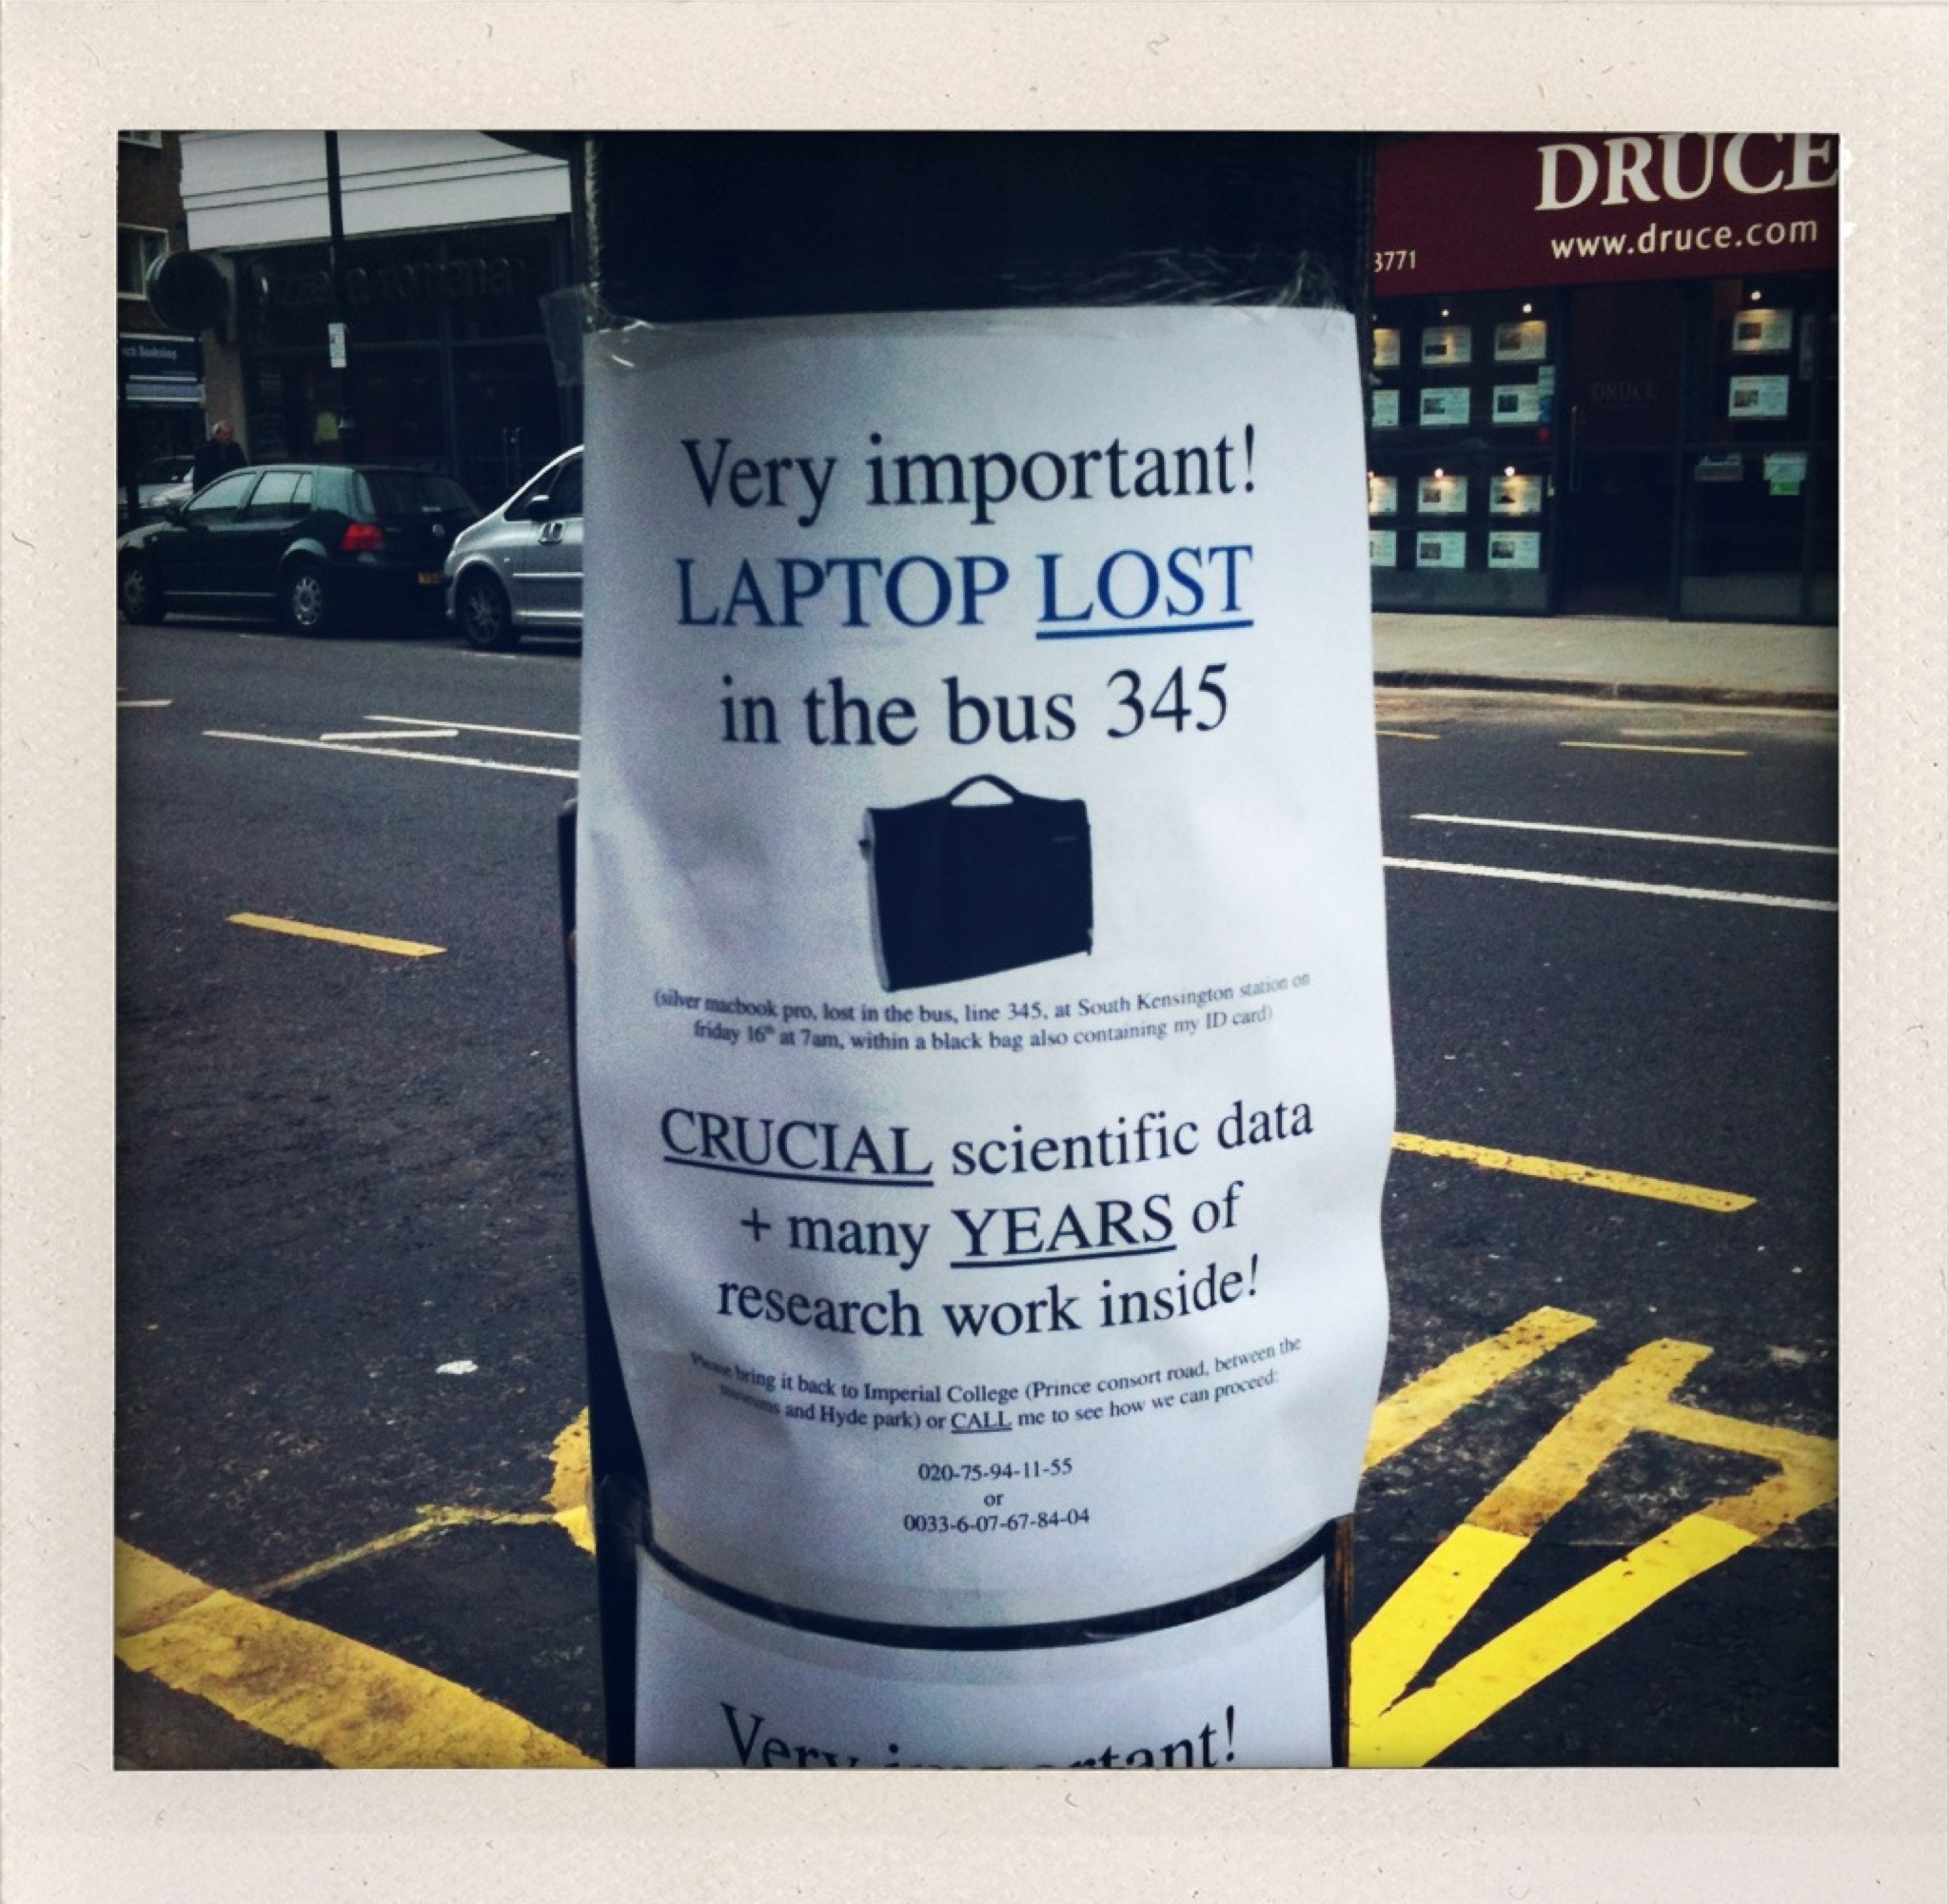
\includegraphics[width=\textwidth]{images/lost_laptop.png}
      \caption{Carelessness.}
    \end{subfigure}
    \hfill
    \begin{subfigure}[b]{0.3\textwidth}
      \centering
      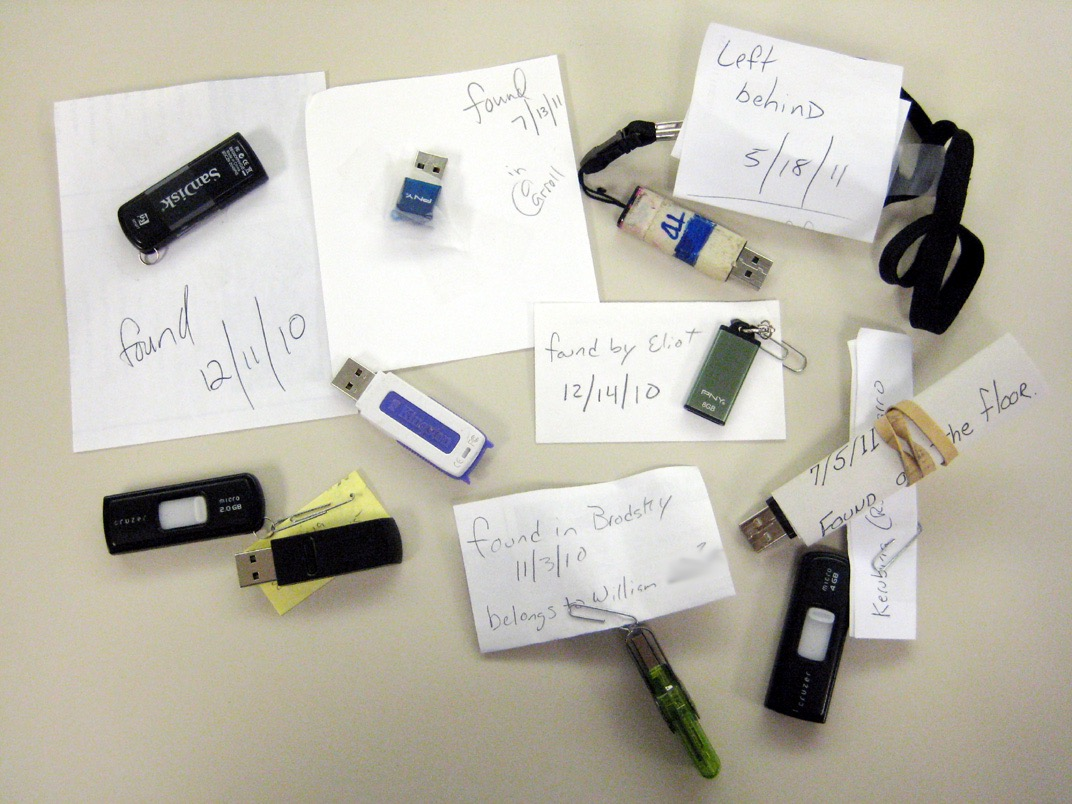
\includegraphics[width=\textwidth]{images/lost_usb_stick.png}
      \caption{Handling.}
    \end{subfigure}
    \hfill
    \begin{subfigure}[b]{0.3\textwidth}
      \centering
      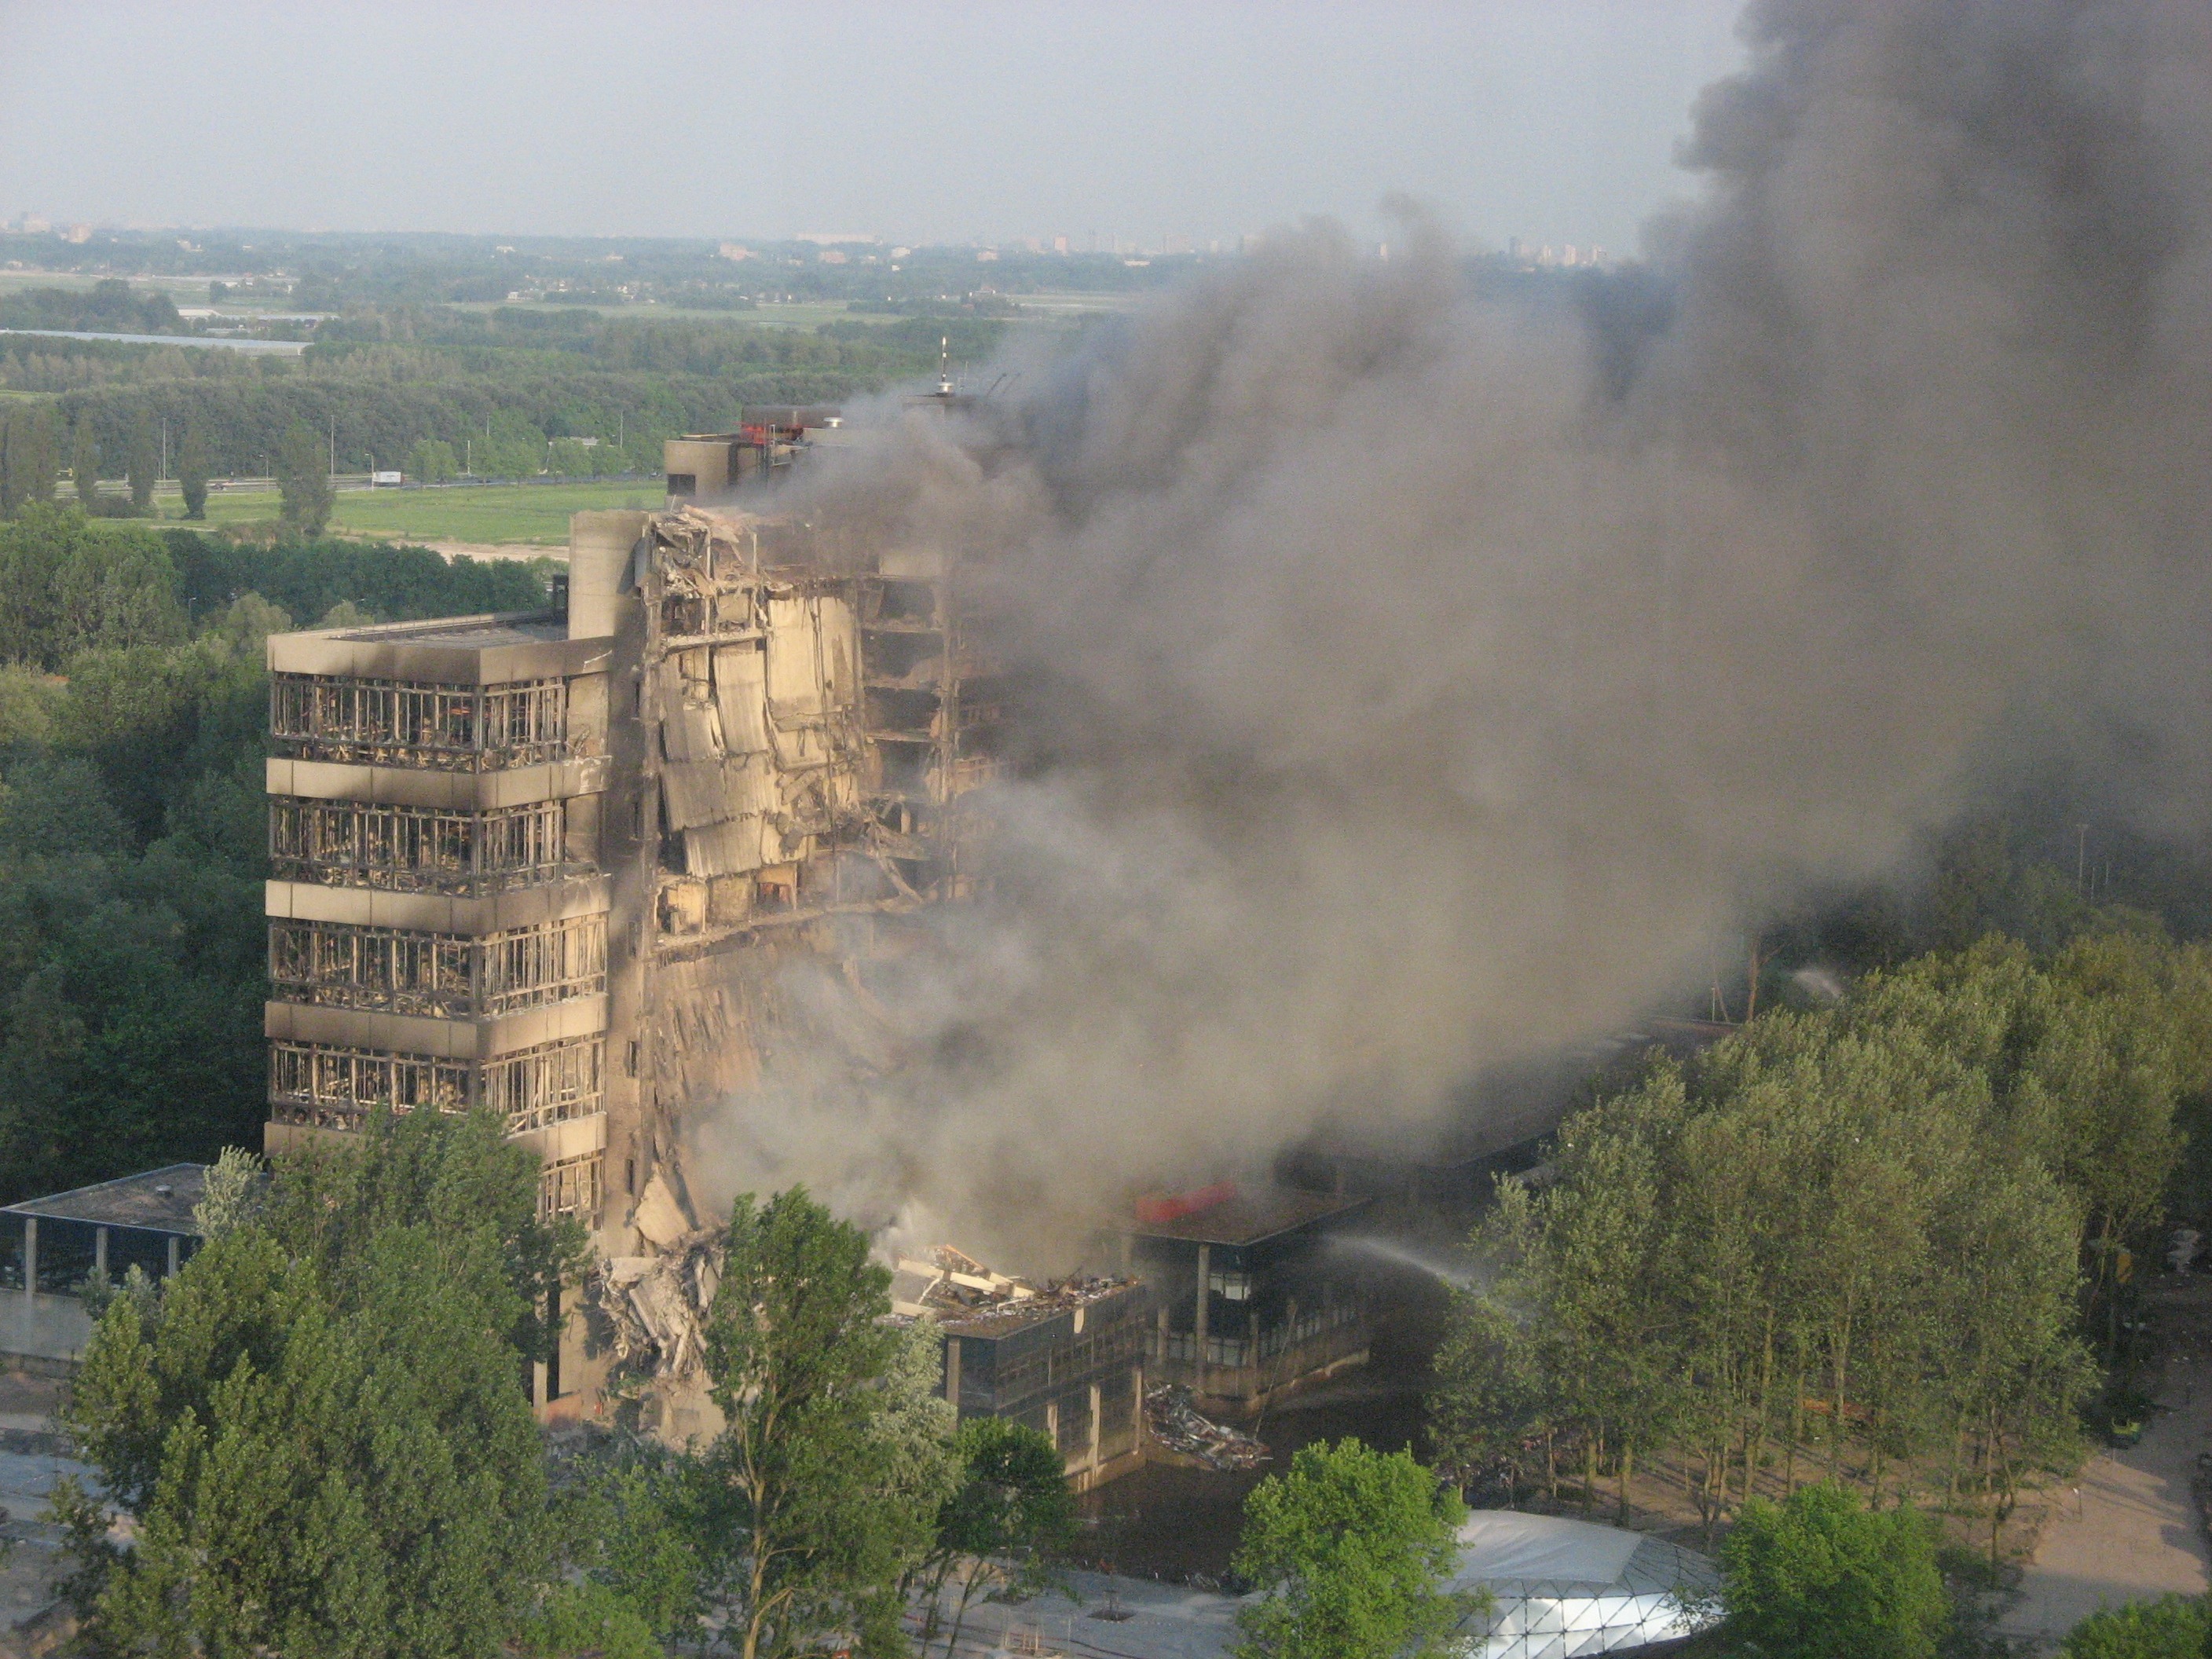
\includegraphics[width=\textwidth]{images/lost_building.png}
      \caption{Catastrophe.}
    \end{subfigure}
    \caption{Examples of data loss~\cite{nielsen2017}.}
  \end{figure}
\end{frame}

\begin{frame}
  \frametitle{Why use Zenodo?}
  \begin{columns}
    \begin{column}{0.5\textwidth}
      \begin{itemize}
        \item \textbf{Safe}: Data stored at CERN's data centre.
        \item \textbf{Trusted}: Operated by CERN.
        \item \textbf{No waiting time}: Available as soon as published.
        \item \textbf{Open or closed}: Restricted access mode.
        \item \textbf{Usage statistics}.
        \item \textbf{Versioning}: Update data and version numbers.
        \item \textbf{GitHub integration}: Preserve code.
        \item \textbf{Citeable}: Every upload has a DOI.
        \item \textbf{Data principles}: Findable, Accessible, Interoperable, Reusable.
      \end{itemize}
    \end{column}
    \begin{column}{0.5\textwidth}
      \begin{figure}
        \centering
        \includegraphics[scale=0.035]{logos/CERN-logo.png}
        
\includegraphics[scale=0.025]{logos/GitHub-Logo.png}
      \end{figure}
    \end{column}
  \end{columns}
\end{frame}

\begin{frame}
  \frametitle{Research data life cycle}
  \begin{figure}
    \centering
    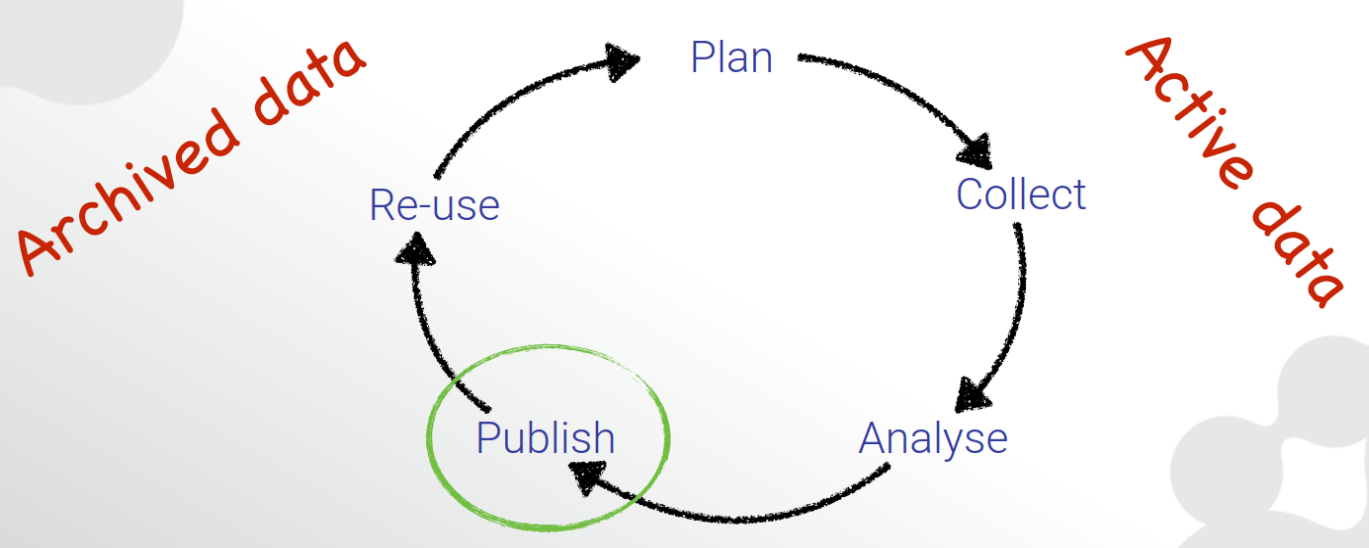
\includegraphics[scale=0.3]{images/zenodo_research_data_lifecycle.png}
    \caption{Research data life cycle according to
    ~\citeauthor{nielsen2017}~\cite{nielsen2017}.}
  \end{figure}
\end{frame}

\begin{frame}
  \frametitle{How do you do it?}
  \begin{columns}
    \begin{column}{0.5\textwidth}
      Sharing your data and software on Zenodo in 3
      steps~\cite{nielsen2017}:
      \begin{enumerate}
        \item Upload.
        \item Describe.
        \item Publish.
      \end{enumerate}
      By the way, the documents cited here, are themselves hosted at Zenodo!
    \end{column}
    \begin{column}{0.5\textwidth}
      \begin{figure}
        \centering
        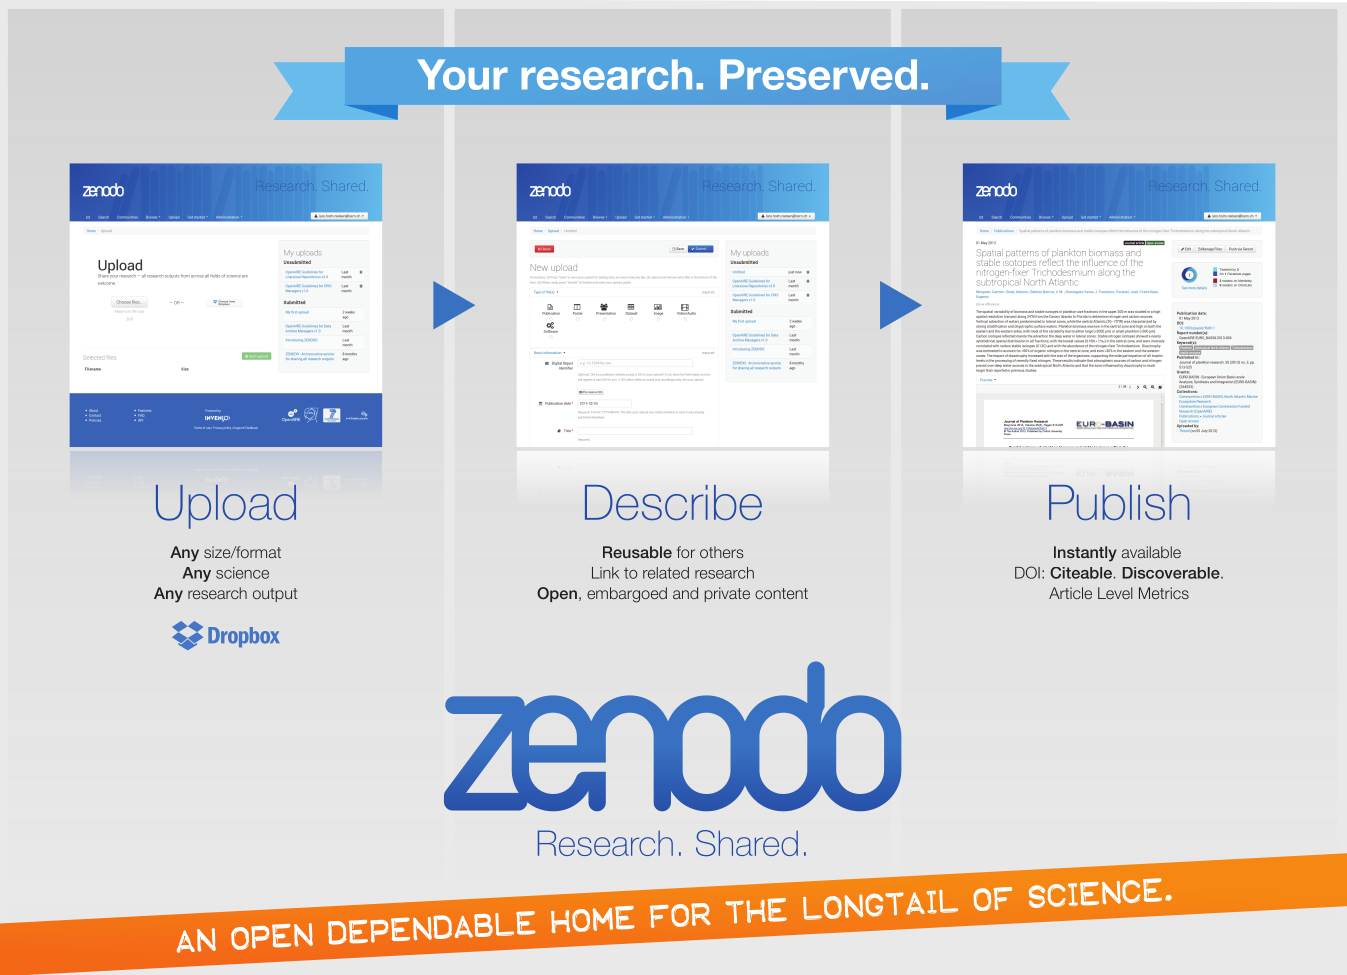
\includegraphics[scale=0.15]{images/zenodo_upload_describe_publish.png}
        \caption{Source: Poster presented in Dublin~\cite{nielsen2014}.}
      \end{figure}
    \end{column}
  \end{columns}
\end{frame}

\begin{frame}
  \frametitle{Upload}
  \begin{columns}
    \begin{column}{0.5\textwidth}
      Before you upload, think about:
      \begin{itemize}
        \item Data management plan.
        \item File formats (open versus proprietary).
        \item Standards.
        \item Re-usability.
        \item Licenses.
        \item Privacy.
      \end{itemize}
    \end{column}
    \begin{column}{0.5\textwidth}
      Zenodo allows:
      \begin{itemize}
        \item Any format.
        \item Any licence.
        \item Maximum of 50GB* and 100 files per dataset.
        \item Drag and drop upload.
      \end{itemize}
    \end{column}
  \end{columns}
\end{frame}

\begin{frame}
  \frametitle{Describe}
  \begin{columns}
    \begin{column}{0.5\textwidth}
      Basic information:
      \begin{itemize}
        \item Community (e.g. \textit{treeslab}).
        \item Authors or creators.
        \item Type: Dataset, image, model, poster, presentation, publication
          (book, chapter, conference paper or proceeding, report), software
          (notebook), video, audio.
        \item Title.
        \item Licenses.
      \end{itemize}
    \end{column}
    \begin{column}{0.5\textwidth}
      Recommended information:
      \begin{itemize}
        \item Contributors.
        \item Keywords and subjects.
        \item Dates.
        \item Version.
        \item Publisher.
      \end{itemize}
      Other information:
      \begin{itemize}
        \item Funding, alternate identifiers, related works, references,
          software, publishing information, conference, domain specific fields,
          visibility (public or restricted-embargo).
      \end{itemize}
    \end{column}
  \end{columns}
\end{frame}

\begin{frame}
  \frametitle{Publish}
  \begin{itemize}
    \item Files are not editable.
    \item Metadata is editable.
  \end{itemize}
\end{frame}

\subsection{Zenodo and TREESLab}

\begin{frame}
  \frametitle{TREESLab community at Zenodo}
  \begin{columns}
    \begin{column}{0.5\textwidth}
      \begin{itemize}
        \item You can publish any data to your Zenodo account.
        \item But you can also submit your data to the
          \href{https://tinyurl.com/treeslab-zenodo}{TREES' community}.
        \item This community accepts datasets related to publications produced
          by the TREES lab.
        \item Submissions are reviewed for quality and compliance to TREES
          standards.
      \end{itemize}
    \end{column}
    \begin{column}{0.5\textwidth}
      \centering
      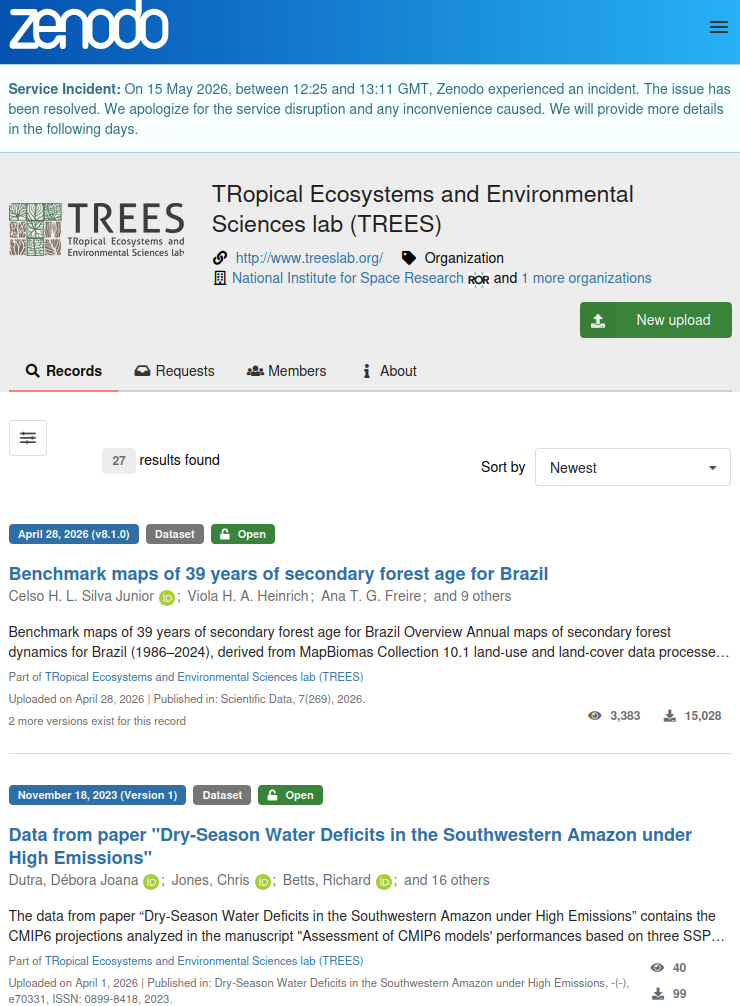
\includegraphics[scale=0.2]{images/zenodo_community_treeslab.png}
    \end{column}
  \end{columns}
\end{frame}

\begin{frame}
  \begin{figure}
    \centering
    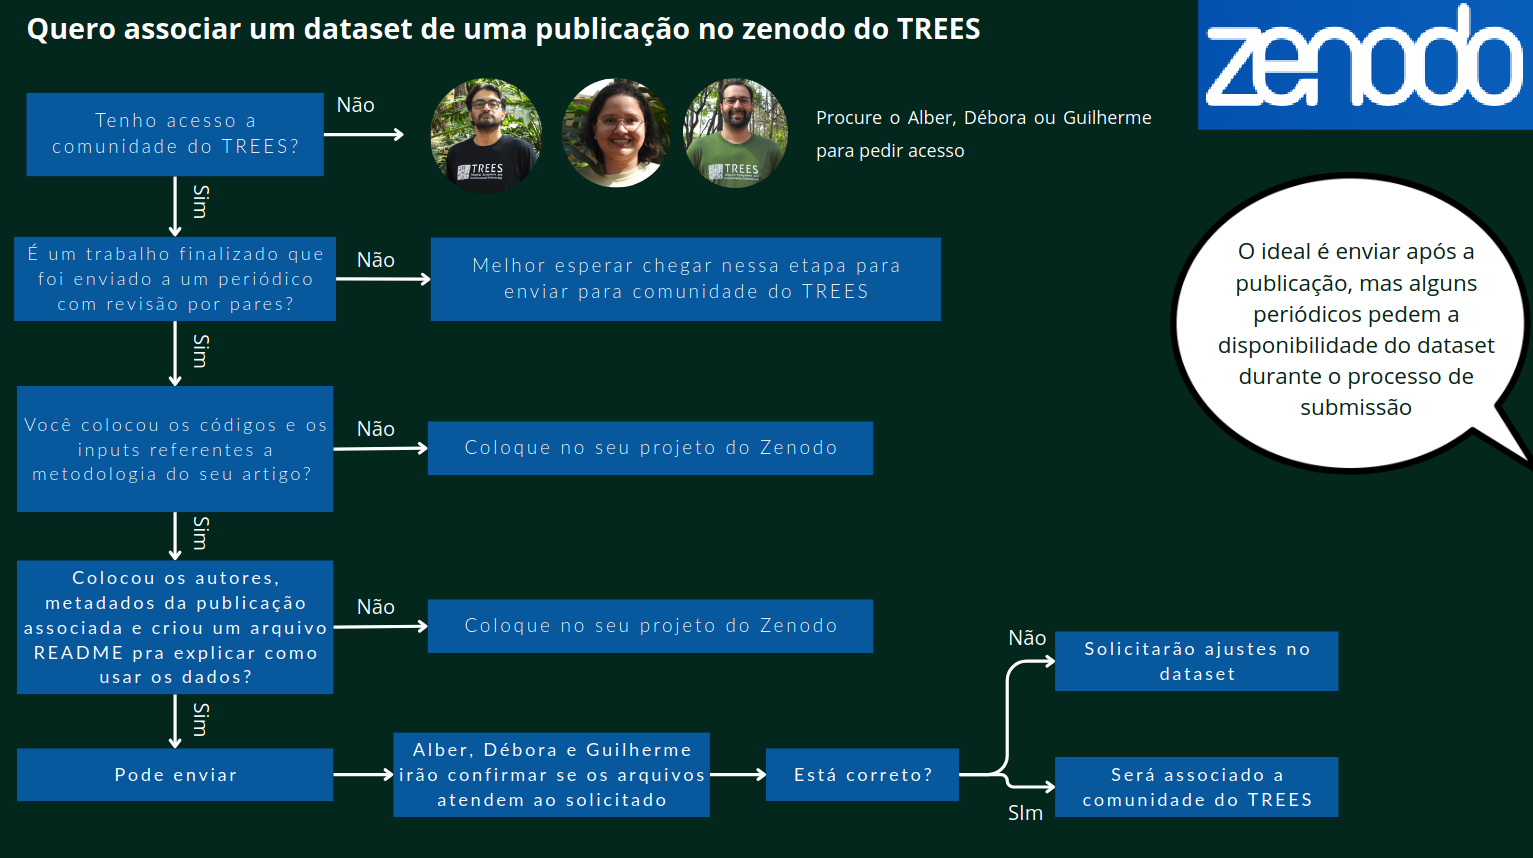
\includegraphics[scale=0.275]{images/zenodo_treeslab_add.png}
  \end{figure}
\end{frame}

\begin{frame}
  \frametitle{TREES' check list for Zenodo}
  \begin{columns}
    \begin{column}{0.5\textwidth}
      \begin{itemize}
        \item You \textbf{must} have an Zenodo account associated to TREES'
          community to submit datasets to this community.
        \item Your submission would be peer rewiewed by TREES' members (A + R
          in the \href{https://tinyurl.com/treeslab-membros}{RACI matrix}).
        \item To avoid common pitalls, we prepared a 
          (\href{https://docs.google.com/document/d/18ZKzcsP6GazzO0X5FDE8FUfkehaD3X3hoxrnWLSxI8o/edit?usp=sharing}
          {check list}).
        \item Read the check list before submitting your dataset to the TREES'
          community at Zenodo.
      \end{itemize}
    \end{column}
    \begin{column}{0.5\textwidth}
       Common recommendations include:
      \begin{itemize}
        \item Add a README.pdf file, describing the files in your submission.
        \item Your submission's name \textbf{must} start with
          \textit{"Data from ..."} or \textit{"Code for ..."}.
        \item Include the name of financing agencies (e.g. FAPESP, CAPES,
          CNPq).
        \item Fill in ZENODO's metadata fields: description, keywords, license,
          link to a publication.
      \end{itemize}
    \end{column}
  \end{columns}
\end{frame}

\begin{frame}
  Questions
  \begin{itemize}
    \item \textit{Qual o formato padrão proposto pelo Trees para o Zenodo.}
    \item \textit{Uma noção básica do funcionamento da plataforma.}
  \end{itemize}
\end{frame}
